% preambulo %%%%%%%%%%%%%%%%%%%%%%%%%%%%%%%%%%%%%%%%%%%%%%%%%%%%%%
\documentclass[a4paper,10pt]{article} %twocolumn
\usepackage[utf8]{inputenc} % letras acentuadas
\usepackage[portuguese]{babel} % tradução de títulos
\usepackage{algorithm} % ambiente para índice de algoritmos
\usepackage{algpseudocode} % fonte e estilo do algoritmo
\usepackage{graphicx}
% \usepackage{natbib}
%[noend]

\floatname{algorithm}{Algoritmo} % tradução da palavra algorítimo no ambiente de índice

% capa %%%%%%%%%%%%%%%%%%%%%%%%%%%%%%%%%%%%%%%%%%%%%%%%%%%%%%
\title{Comparando os algoritmos de ordenação}
\author{Ruben Carlo Benante \\ Autor2 \\ Autor3}

\begin{document}

\maketitle

% resumo %%%%%%%%%%%%%%%%%%%%%%%%%%%%%%%%%%%%%%%%%%%%%%%%%%%%%%
\begin{abstract}

Vamos comparar os algoritmos \textit{xsort} e \textit{ysort} para bla bla.
Para compilar o PDF a partir do TEX use o comando:

\begin{enumerate}
 \item \texttt{pdflatex exN.tex -o exN.pdf}
 \item \texttt{bibtex exN}
 \item \texttt{pdflatex exN.tex -o exN.pdf}
\end{enumerate}

Este é o fim do resumo.

\end{abstract}


% artigo %%%%%%%%%%%%%%%%%%%%%%%%%%%%%%%%%%%%%%%%%%%%%%%%%%%%%%
% seção de introdução %%%%%%%%%%%%%%%%%%%%%%%%%%%%%%%%%%%%%%%%%%%%%%%%%%%%%%
\section{Introdução ao métodos de ordenação}

Métodos de ordenação tem a principal função de...

O algoritmo \textit{Tal-e-qual} trabalha percorrendo uma árvore tal tal e tal.

% seção do primeiro algoritmo %%%%%%%%%%%%%%%%%%%%%%%%%%%%%%%%%%%%%%%%%%%%%%%%%%%%%%
\section{O \textit{BubbleSort}}

O algoritmo \emph{Xsort} trabalha fazendo uma varredura na ...

\begin{figure}[ht]
\centering
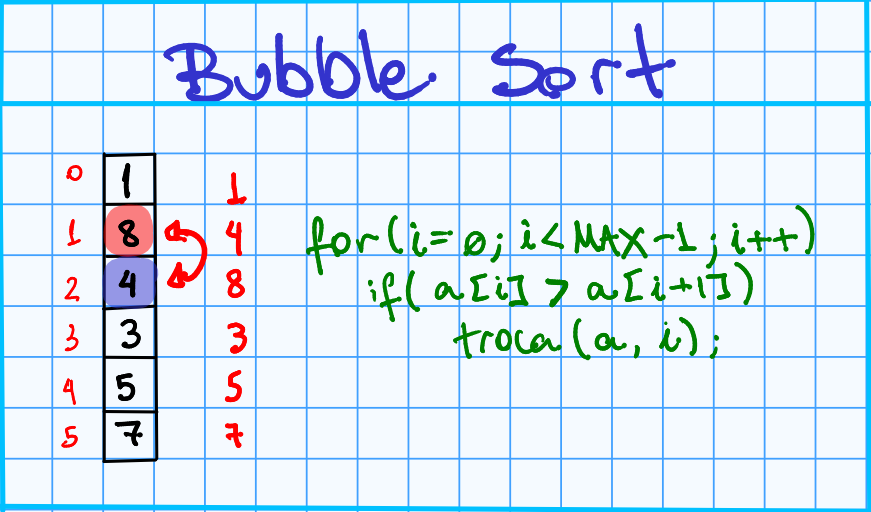
\includegraphics[width=.80\linewidth]{bubble.png}
\caption{Exemplo de ordenação com Bubblesort}
\label{fig:xsort}
\end{figure}


% subseção com algoritmo %%%%%%%%%%%%%%%%%%%%%%%%%%%%%%%%%%%%%%%%%%%%%%%%%%%%%%
\subsection{Implementação}

O algoritmo é descrito abaixo:

% seção do segundo algoritmo %%%%%%%%%%%%%%%%%%%%%%%%%%%%%%%%%%%%%%%%%%%%%%%%%%%%%%
\section{O \textit{QuickSort}}

O método \emph{Ysort} é caracterizado por...


% subseção com algoritmo %%%%%%%%%%%%%%%%%%%%%%%%%%%%%%%%%%%%%%%%%%%%%%%%%%%%%%
\subsection{Implementação}

Para conseguir blablabla

O algoritmo \textit{Ysort} segue abaixo:

\begin{algorithm}
\caption{Algoritmo Ysort}\label{alg:ysort}
\begin{algorithmic}[1]
\Function{ysort}{estado}\Comment{retorna uma ação}
\State \textbf{Entradas}: estado é a configuração atual do jogo
\State $v\gets \mathrm{maxvalor}{(estado)}$
\State \textbf{returna} a ação $a$ em sucessores(estado) cujo valor é $v$ %\Comment{comentario}
% \While{$r\not=0$}\Comment{We have the answer if r is 0}
% \State $a\gets b$
% \State $b\gets r$
% \State $r\gets a\bmod b$
% \EndWhile\label{euclidendwhile}
\EndFunction
\Function{maxvalor}{estado}\Comment{retorna o valor estático}
\If{fim(estado)}
   \State \textbf{retorna} estatico(estado)
\EndIf
\State $v \gets -\infty$
\For{todas ações $a$ nos sucessores(estado)}
    \State $v \gets \max{(v, \mathrm{minvalor}(a))}$
\EndFor
\State \textbf{retorna} $v$
\EndFunction
\Function{minvalor}{estado}\Comment{retorna o valor estático}
\If{fim(estado)}
   \State \textbf{retorna} estatico(estado)
\EndIf
\State $v \gets \infty$
\For{todas ações $a$ nos sucessores(estado)}
    \State $v \gets \min{(v, \mathrm{maxvalor}(a))}$
\EndFor
\State \textbf{retorna} $v$
\EndFunction
\end{algorithmic}
\end{algorithm}

% seção onde se faz a comparação %%%%%%%%%%%%%%%%%%%%%%%%%%%%%%%%%%%%%%%%%%%%%%%%%%%%%%
\section{Comparando \textit{XSort} o \textit{YSort}}

% método utilizado %%%%%%%%%%%%%%%%%%%%%%%%%%%%%%%%%%%%%%%%%%%%%%%%%%%%%%
\subsection{Método}

O método usado para comparação foi...

% resultados obtidos %%%%%%%%%%%%%%%%%%%%%%%%%%%%%%%%%%%%%%%%%%%%%%%%%%%%%%
\subsection{Resultados}

Os resultados mostrados na tabela \ref{tab:resultados} demonstram ...

\begin{table}
\begin{center}
 \caption{Tabela de custo de pontos para habilidades}
\begin{tabular}{|l|r|}
  \hline \hline
  pontos & moedas \\ \hline \hline
   8 & 0 \\ \hline
   9 & 1 \\ \hline
  10 & 2 \\ \hline
  11 & 3 \\ \hline
  12 & 4 \\ \hline
  13 & 5 \\ \hline
  14 & 7 \\ \hline
  15 & 9 \\ \hline \hline
\end{tabular} 
\label{tab:resultados}
\end{center}
\end{table}


% seção de conclusão %%%%%%%%%%%%%%%%%%%%%%%%%%%%%%%%%%%%%%%%%%%%%%%%%%%%%%
\section{Conclusão do artigo}

    Concluimos,com base nos estudos e testes coletados sobre os algoritmos de ordenação propostos, que para fins educacionais, o algoritmo \textit{BubbleSort} é mais indicado devido a sua simples implementação, cabendo então para o \textit{QuickSort} ser o mais indicado entre os dois, quando requer uma demanda em menor tempo e com mais eficiência.

De acordo com \cite{Benante2008phd}, este é o fim do artigo.

%%%%%%%%%%%%%%%%%%%%%%%%%%%%%%%%%%%%%%%%%%%%%%%%%%%%%%%%%%%%%%%%%%%%%%%%%%%%%%%%%%%%%%%%%%%%%%%%%%%%%%%%%%%%
% referências bibliográficas %%%%%%%%%%%%%%%%%%%%%%%%%%%%%%%%%%%%%%%%%%%%%%%%%%%%%%
%\section*{Referências Bibliográficas}

% cite todos, mesmo os não referenciados %%%%%%%%%%%%%%%%%%%%%%%%%%%%%%%%%%%%%%%%%%%%%%%%%%%%%%
\nocite{*}

% se necessario %%%%%%%%%%%%%%%%%%%%%%%%%%%%%%%%%%%%%%%%%%%%%%%%%%%%%%
% troca autor and autor por autor & autor, na bibliografia. O dcu usa "and"
%\renewcommand{\harvardand}{\&} % troca and pro &. O dcu usa "and"

% Estilos de bibliografia %%%%%%%%%%%%%%%%%%%%%%%%%%%%%%%%%%%%%%%%%%%%%%%%%%%%%%
% \bibliographystyle{abnt-alf} % Estilo alfabético da ABNT. Opção [num] para estilo numérico
%\bibliographystyle{apalike}
%\bibliographystyle{dcu} %citacao como (autor and autor, ano). Parece apalike. Rev. Control. Automacao. Use com harvard
%\bibliographystyle{agsm} % padrao harvard fica (autor & autor ano).
\bibliographystyle{acm}

% arquivo de banco de dados das referências %%%%%%%%%%%%%%%%%%%%%%%%%%%%%%%%%%%%%%%%%%%%%%%%%%%%%%
% renomear para o número do exercício correto
% o arquivo de bibliografia pode se chamar qualquer coisa, isso não muda o comando de gerar o PDF. 
% Por exemplo para 'mybiblio.bib', use \bibliography{mybiblio} e os comandos pdflatex e bibtex continuam os mesmos identicos com exN.
\bibliography{exN}

\end{document}
